\chapter{Arhitektura i dizajn sustava}
		
	Arhitektura se moze podijeliti na tri podsustava:
	
	\begin{itemize}
		\item Web posluzitelj
		\item Web aplikacija
		\item Baza podataka
	\end{itemize}

	
	\textit{Web preglednik} je alat koji omogućava korisnicima pregledavanje web stranica i njihovih povezanih multimedijalnih sadržaja. Svaki internetski preglednik djeluje kao prevoditelj, jer interpretira web stranice napisane u kodu kako bi ih prikazao korisnicima na razumljiv način. Korisnici putem web preglednika šalju zahtjeve web poslužitelju.
	
	\textit{Web poslužitelj} je ključni element u radu web aplikacije. Njegova glavna uloga je olakšavanje komunikacije između klijenta i aplikacije putem HTTP protokola. Poslužitelj pokreće web aplikaciju i prenosi joj zahtjev.
	
	\textit{Web aplikacija} služi korisniku za obradu željenih zahtjeva. Aplikacija obrađuje zahtjev, pristupa bazi podataka prema potrebi i putem poslužitelja vraća korisniku odgovor u obliku HTML dokumenta koji se prikazuje u web pregledniku.
	
	\textit{Baza podataka} ima svrhu pohranjivanja i upravljanja strukturiranim podacima koji se koriste u aplikaciji. Svaki put kad korisnik šalje zahtjev putem web preglednika, web aplikacija može pristupiti bazi podataka kako bi dohvatila ili ažurirala potrebne informacije. Baza podataka omogućava učinkovit pristup, pretraživanje i manipulaciju podacima, što je ključno za pravilan rad web aplikacije.
	
	Za izradu naše web aplikacije odabrali smo programski jezik Java zajedno s Springboot radnim okvirom, kao i programski jezik JavaScript. Razvojna okruženja koja koristimo su Visual Studio Code i IntelliJ. Arhitektura sustava temelji se na MVC (Model-View-Controller) konceptu, koji je podržan od strane Springboot radnog okvira i nudi gotove predloške koji olakšavaju razvoj web aplikacije. Kao poslužitelja baze podataka smo koristili PostgreSQL.
	
	MVC koncept donosi neovisnost u razvoju pojedinih dijelova aplikacije, što olakšava testiranje, kao i dodavanje novih svojstava u sustav. Sastoji se od:
	
	\begin{itemize}
		\item \textbf{Model} - Središnja komponenta sustava koja predstavlja dinamičke strukture podataka neovisne o korisničkom sučelju. Upravlja podacima, logikom i pravilima aplikacije, te prima ulazne podatke od Controllera.
		\item \textbf{View} - Ovdje se prikazuju podaci, primjerice u obliku grafova. Moguća su različita sučelja za prikaz informacija, poput grafičkog ili tabličnog prikaza podataka.
		\item \textbf{Controller} - Prima ulaze i prilagođava ih za daljnju interakciju s Modelom ili Viewom. Upravlja korisničkim zahtjevima i temeljem njih izvodi daljnje interakcije s ostalim elementima sustava.
	\end{itemize}
		

		

				
		\section{Baza podataka}
				
				Za bazu podataka koristi se relacijska baza podataka koja se sastoji od relacija. Svaka relacija ima svoje ime i atribute. Vrste atributa koji se mogu nalaziti u relaciji su primarni ključ, strani ključ ili atribut s nekom informacijom vezanom za relaciju. Baza podataka sastoji se od relacija:
		
				\begin{packed_item}
					\item AppUser
					\item ConfirmationToken
					\item StationManager
					\item SearcherInTheField
					\item Action
					\item Request
					\item Station
					\item Qualification
					\item Animal
					\item Location
				\end{packed_item}
		
			\subsection{Opis tablica}
			

				U relaciju \textbf{AppUser} pohranjuju se podaci o korisniku: \textit{id, userName, image, firstName, lastName, email, password, locked, enabled}. Primarni ključ je \textit{id}, i nema stranih ključeva. S atributom \textit{id} je u odnosu One-to-One s relacijama \textbf{StationManager} i \textbf{SearcherInTheField} i u odnosu One-to-Many s relacijama \textbf{ConfirmationToken} i \textbf{Action}.
				
				
				\begin{longtblr}[
					label=none,
					entry=none
					]{
						width = \textwidth,
						colspec={|X[6,l]|X[6, l]|X[20, l]|}, 
						rowhead = 1,
					} %definicija širine tablice, širine stupaca, poravnanje i broja redaka naslova tablice
					\hline \SetCell[c=3]{c}{\textbf{AppUser}}	 \\ \hline[3pt]
					\SetCell{LightGreen}id & BIGINT	&  	id korisnika 	\\ \hline
					userName	& VARCHAR &  korisničko ime 	\\ \hline 
					image & BYTEA &  heksadekatski zapis korisničke slike  \\ \hline 
					firstName & VARCHAR	&  ime korisnika  \\ \hline 
					lastName & VARCHAR	&  prezime korisnika  \\ \hline 
					email & VARCHAR	&  email korisnika  \\ \hline 
					password & VARCHAR	&  lozinka korisnika  \\ \hline 
					locked & BOOLEAN & je li korisnika potvrdio admin \\ \hline
					enabled & BOOLEAN & je li korisnik potvrđen emailom \\ \hline
				\end{longtblr}
				
				U relaciju \textbf{ConfirmationToken} pohranjuju se podaci: \textit{id, token, createdAt, expiresAt, confirmedAt, user}. Primarni ključ je \textit{id}, a strani ključ je \textit{user}. S atributom \textit{user} je u odnosu Many-to-One s relacijom \textbf{AppUser}.
				
				\begin{longtblr}[
					label=none,
					entry=none
					]{
						width = \textwidth,
						colspec={|X[6,l]|X[6, l]|X[20, l]|}, 
						rowhead = 1,
					} %definicija širine tablice, širine stupaca, poravnanje i broja redaka naslova tablice
					\hline \SetCell[c=3]{c}{\textbf{ConfirmationToken}}	 \\ \hline[3pt]
					\SetCell{LightGreen}id & BIGINT	&  	id tokena 	\\ \hline
					token & VARCHAR & token \\ \hline
					createdAt & TIMESTAMP & vrijeme kada je token stvoren \\ \hline
					expiersAt & TIMESTAMP & vrijeme kada token ističe \\ \hline
					confirmedAt & TIMESTAMP & vrijeme kada je token potvrđen \\ \hline
					\SetCell{LightBlue}user	& BIGINT &  id korisnika kojemu je poslan token \\ \hline  
				\end{longtblr}

				U relaciju \textbf{StationManager} pohranjuju se podaci: \textit{id, station}. Primarni ključ i ujedno i strani ključ je \textit{id} i također je strani ključ \textit{station}. S atributom \textit{id} je u odnosu One-to-One s relacijom \textbf{AppUser}, s atributom \textit{station} je u odnosu One-to-One s relacijom \textbf{Station}.
				
				\begin{longtblr}[
					label=none,
					entry=none
					]{
						width = \textwidth,
						colspec={|X[6,l]|X[6, l]|X[20, l]|}, 
						rowhead = 1,
					} %definicija širine tablice, širine stupaca, poravnanje i broja redaka naslova tablice

					\hline \SetCell[c=3]{c}{\textbf{StationManager}}	 \\ \hline[3pt]
					\SetCell{LightGreen}id & BIGINT	&  	id korisničkog računa voditelja 	\\ \hline
					\SetCell{LightBlue}station & BIGINT	&  	id postaje koju vodi voditelj 	\\ \hline
				\end{longtblr}
			
			U relaciju \textbf{SearcherInTheField} pohranjuju se podaci: \textit{id, station, qualification}. Primarni ključ i ujedno i strani ključ je \textit{id} i također je strani ključ \textit{station} i \textit{qualification}. S atributom \textit{id} je u odnosu One-to-One s relacijom \textbf{AppUser}, s atributom \textit{station} je u odnosu Many-to-One s relacijom \textbf{Station}, s atributom \textit{qualification} je u odnosu Many-to-One s relacijom \textbf{Qualification}, s atributom \textit{id} je u odnosu One-to-Many s relacijom \textbf{Request} i  s atributom \textit{id} je u odnosu One-to-Many s relacijom \textbf{Location}.

			
				\begin{longtblr}[
					label=none,
					entry=none
					]{
						width = \textwidth,
						colspec={|X[10,l]|X[6, l]|X[20, l]|}, 
						rowhead = 1,
					} %definicija širine tablice, širine stupaca, poravnanje i broja redaka naslova tablice

					\hline \SetCell[c=3]{c}{\textbf{SearcherInTheField}}	 \\ \hline[3pt]
					\SetCell{LightGreen}id & BIGINT	&  	id korisničkog računa tragača 	\\ \hline
					\SetCell{LightBlue}station & BIGINT	&  	id postaje kojoj pripada 	\\ \hline
					\SetCell{LightBlue}qualification	& BIGINT &  id osposobljenosti tragača 	\\ \hline  
				\end{longtblr}
			
			U relaciju \textbf{Action} pohranjuju se podaci: \textit{id, begun, description, comment}. Primarni ključ je \textit{id}, strani ključ je \textit{begun}. S atributom \textit{begun} je u odnosu Many-to-One s relacijom \textbf{AppUser} i s atributom \textit{id} je u odnosu One-to-Many s relacijom \textbf{Request}.

			
			\begin{longtblr}[
				label=none,
				entry=none
				]{
					width = \textwidth,
					colspec={|X[6,l]|X[6, l]|X[20, l]|}, 
					rowhead = 1,
				} %definicija širine tablice, širine stupaca, poravnanje i broja redaka naslova tablice
				
				\hline \SetCell[c=3]{c}{\textbf{Action}}	 \\ \hline[3pt]
				\SetCell{LightGreen}id & BIGINT	&  	id akcije 	\\ \hline
				\SetCell{LightBlue}begun & BIGINT	&  	id korisnika (istraživača) koji je započeo akciju 	\\ \hline
				description	& TEXT &  opis akcije 	\\ \hline
				comment & TEXT &  komentar za akciju 	\\ \hline  
			\end{longtblr}
			
			U relaciju \textbf{Request} pohranjuju se podaci: \textit{id, action, searcher, description, qualification, completed}. Primarni ključ je \textit{id}, strani ključevi su \textit{action}, \textit{searcher} i \textit{qualification}. S atributom \textit{action} je u odnosu Many-to-One s relacijom \textbf{Action}, s atributom \textit{searcher} je u odnosu Many-to-One s relacijom \textbf{SearcherInTheField} i s atributom \textit{qualification} je u odnosu One-to-One s relacijom \textbf{Qualification}.

			
			\begin{longtblr}[
				label=none,
				entry=none
				]{
					width = \textwidth,
					colspec={|X[6,l]|X[6, l]|X[20, l]|}, 
					rowhead = 1,
				} %definicija širine tablice, širine stupaca, poravnanje i broja redaka naslova tablice

				\hline \SetCell[c=3]{c}{\textbf{Request}}	 \\ \hline[3pt]
				\SetCell{LightGreen}id & BIGINT	&  	id zahtjeva 	\\ \hline
				\SetCell{LightBlue}action & BIGINT	&  	id akcije kojoj pripada zahtjev 	\\ \hline
				\SetCell{LightBlue}searcher & BIGINT	&  	id tragača koji je dobio zahtjev 	\\ \hline
				description	& TEXT &  opis  što tragač mora napraviti 	\\ \hline 
				\SetCell{LightBlue} qualification & TEXT & potrebne kvalifikacije \\ \hline
				completed & BOOLEAN & je li zahtjev završen ili ne \\ \hline
			\end{longtblr}
			
			U relaciju \textbf{Station} pohranjuju se podaci: \textit{id, name}. Primarni ključ je \textit{id} i nema stranih ključeva. S atributom \textit{id} je u odnosu One-to-One s relacijom \textbf{StationManager}, s atributom \textit{id} je u odnosu One-to-Many s relacijom \textbf{SearcherInTheField} i s atributom \textit{id} je u odnosu One-to-One s relacijom \textbf{Location}.

			
			\begin{longtblr}[
				label=none,
				entry=none
				]{
					width = \textwidth,
					colspec={|X[6,l]|X[6, l]|X[20, l]|}, 
					rowhead = 1,
				} %definicija širine tablice, širine stupaca, poravnanje i broja redaka naslova tablice

				\hline \SetCell[c=3]{c}{\textbf{Station}}	 \\ \hline[3pt]
				\SetCell{LightGreen}id & BIGINT	&  	id postaje 	\\ \hline
				name & VARCHAR & ime postaje \\ \hline
			\end{longtblr}
			
			U relaciju \textbf{Qualification} pohranjuju se podaci: \textit{id, description, coverage, visibility}. Primarni ključ je \textit{id} i nema stranih ključeva. S atributom \textit{id} je u odnosu One-to-Many s relacijom \textbf{SearcherInTheField} i u odnosu One-to-One s relacijom \textbf{Request}.

			
			\begin{longtblr}[
				label=none,
				entry=none
				]{
					width = \textwidth,
					colspec={|X[10,l]|X[6, l]|X[20, l]|}, 
					rowhead = 1,
				} %definicija širine tablice, širine stupaca, poravnanje i broja redaka naslova tablice

				\hline \SetCell[c=3]{c}{\textbf{Qualification}}	 \\ \hline[3pt]
				\SetCell{LightGreen}id & BIGINT	&  	id osposobljenost 	\\ \hline
				description & VARCHAR & opis osposobljenosti (npr. pješice, autom,...) \\ \hline
				coverage & DOUBLE PRECISION & područje pokriveno u kilometrima \\ \hline
				visibility & BIGINT & ocjena vidljivosti na skali od 1 do 10 (1 je najgore, a 10 najbolje) \\ \hline
			\end{longtblr}
			
			U relaciju \textbf{Animal} pohranjuju se podaci: \textit{id, species, comment}. Primarni ključ je \textit{id} i nema stranih ključeva. S atributom \textit{id} je u odnosu One-to-Many s relacijom \textbf{Location}.

			
			\begin{longtblr}[
				label=none,
				entry=none
				]{
					width = \textwidth,
					colspec={|X[6,l]|X[6, l]|X[20, l]|}, 
					rowhead = 1,
				} %definicija širine tablice, širine stupaca, poravnanje i broja redaka naslova tablice

				\hline \SetCell[c=3]{c}{\textbf{Animal}}	 \\ \hline[3pt]
				\SetCell{LightGreen}id & BIGINT	&  	id životinje 	\\ \hline
				species & VARCHAR & vrsta životinje \\ \hline
				comment & TEXT & komentar za životinju \\ \hline
			\end{longtblr}
			
			U relaciju \textbf{Location} pohranjuju se podaci: \textit{id, object, longitude, latitude, time, comment}. Primarni ključ je \textit{id}, a strani ključ je \textit{object}. S atributom \textit{object} je u odnosu One-to-One s relacijom \textbf{Station}, Many-to-One s relacijom \textbf{Animal} i Many-to-One s relacijom \textbf{SearcherInTheField}.

			
			\begin{longtblr}[
				label=none,
				entry=none
				]{
					width = \textwidth,
					colspec={|X[6,l]|X[6, l]|X[20, l]|}, 
					rowhead = 1,
				} %definicija širine tablice, širine stupaca, poravnanje i broja redaka naslova tablice

				\hline \SetCell[c=3]{c}{\textbf{Location}}	 \\ \hline[3pt]
				\SetCell{LightGreen}id & BIGINT & id lokacije \\ \hline
				\SetCell{LightBlue}object & BIGINT	&  	id objekta na određenoj lokaciji 	\\ \hline
				longitude & DOUBLE PRECISION & geografska dužina \\ \hline
				latitude & DOUBLE PRECISION & geografska širina \\ \hline
				time & TIMESTAMP & vrijeme kada je lokacija spremljena \\ \hline
				comment & TEXT & komentar za lokaciju \\ \hline

			\end{longtblr}
			
			\subsection{Dijagram baze podataka}
				\begin{figure}[H]
					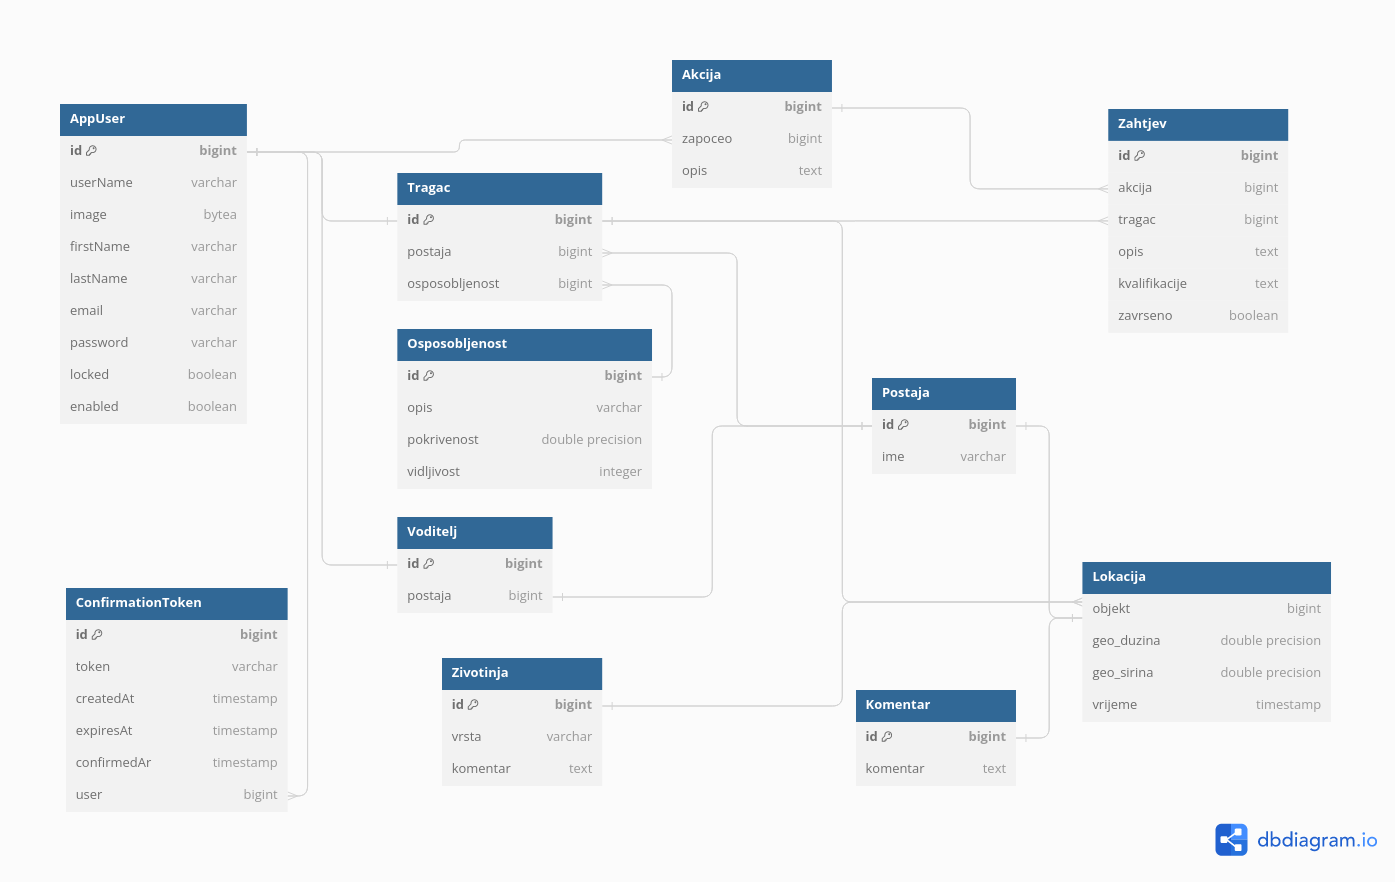
\includegraphics[scale=0.35]{dijagrami/dijagram_baze_podataka.png}
					\centering
					\caption{Dijagram baze podataka}
					\label{fig:promjene}
				\end{figure}
			\eject
			
			
		\section{Dijagram razreda}
		Dijagram razreda podijeljen je zbog bolje preglednosti na tri dijela: Controllers, Models i DTO. Prikazane su veze koje ostvaruju razredi unutar istog dijela dijagrama, a odnosi između razreda u različitim dijelovima mogu se zaključiti iz tipova atributa. Metode korištene u Controller razredima vraćaju \textit{ResponseEntity}, koji predstavlja HTTP odgovor, ili samo kod odgovora HTTP-a. U svom radu koriste objekte za prijenos podataka (DTO) i ostvaruju komunikaciju s klijentskom stranom.
			
			\begin{figure}[H]
				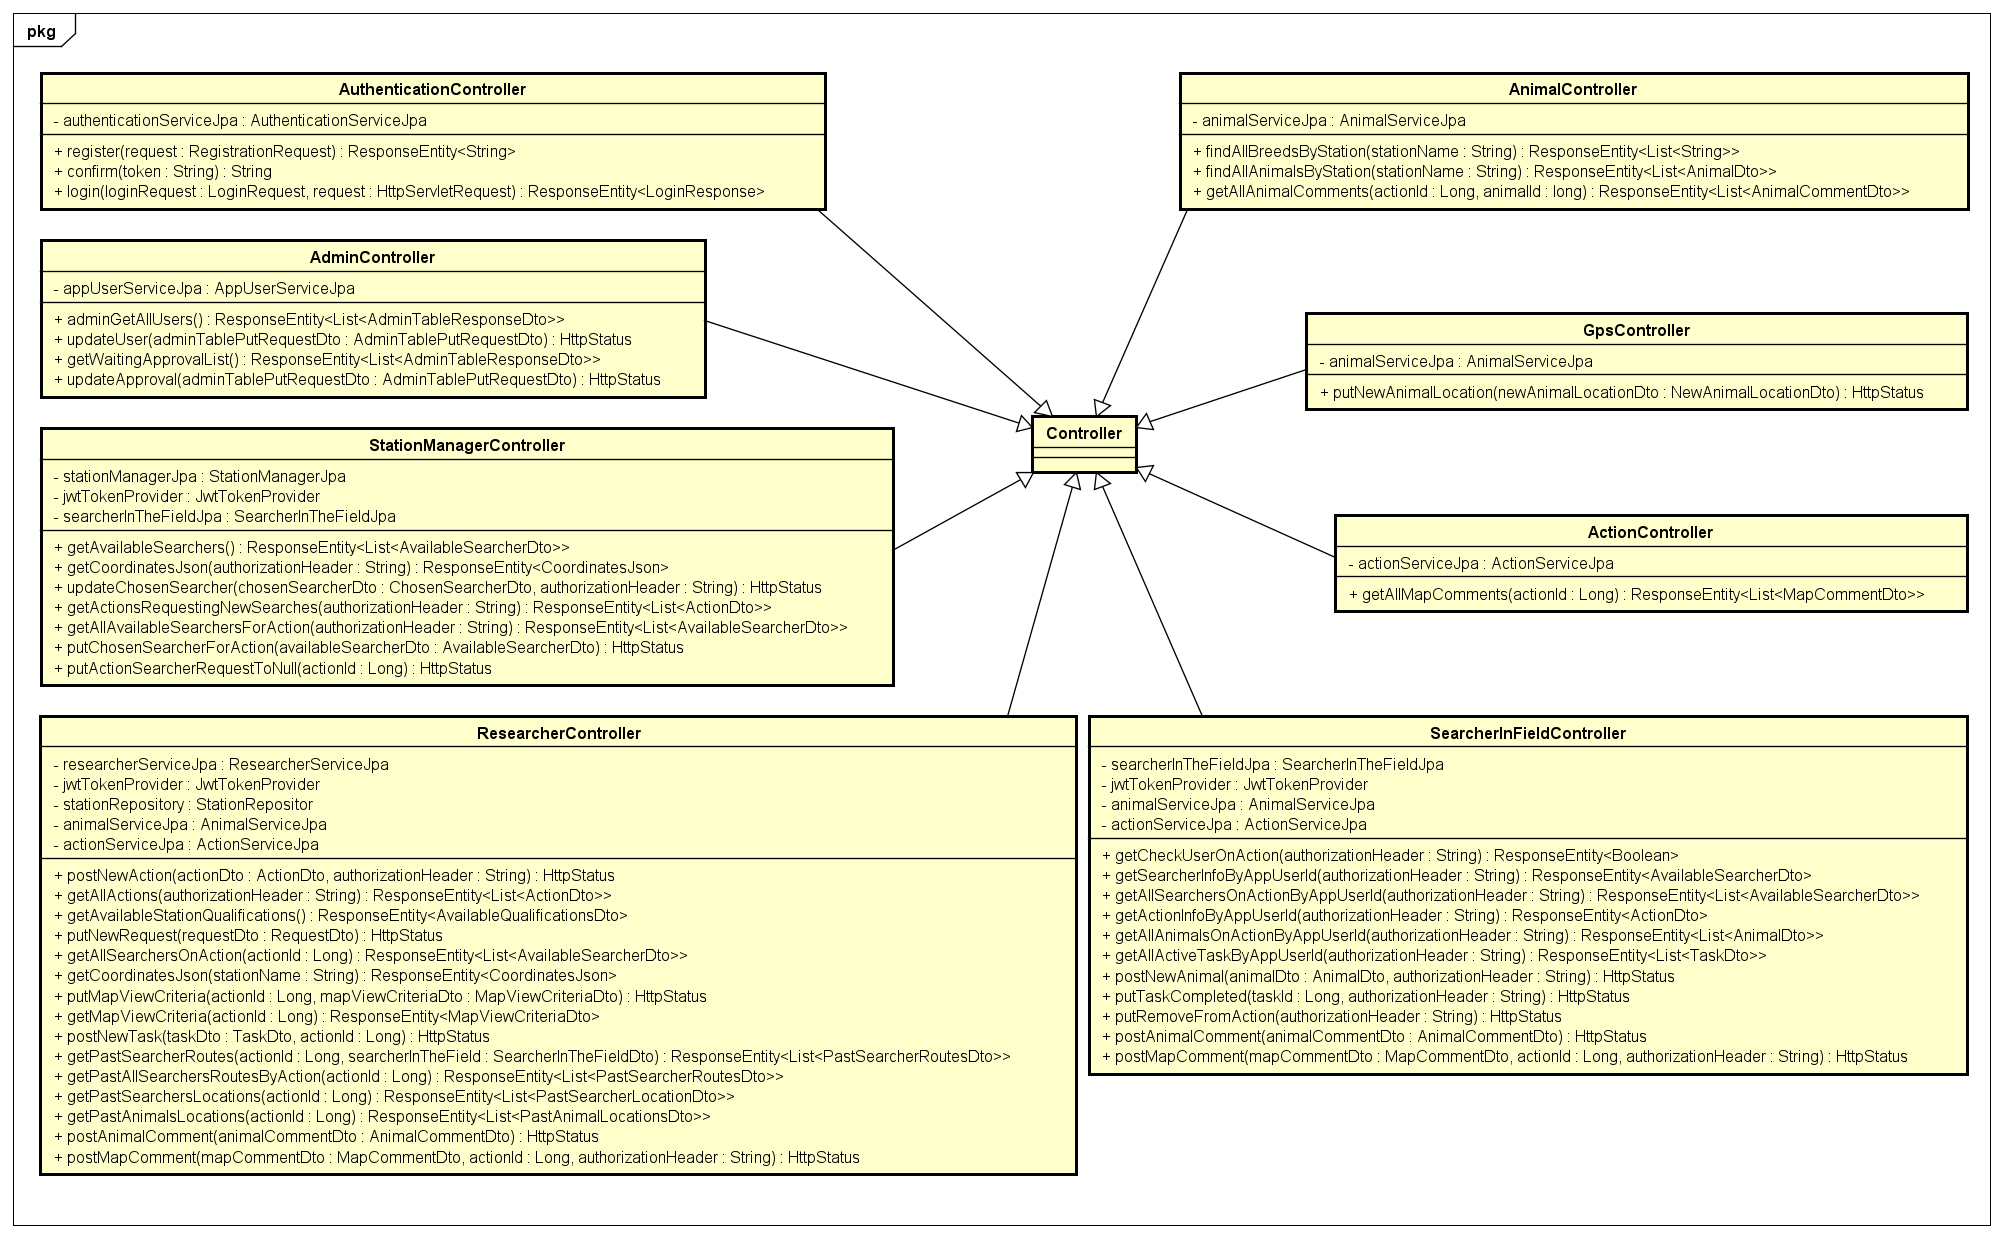
\includegraphics[scale=0.5]{dijagrami/Controllers.png} 
				\centering
				\caption{Dijagram razreda - dio Controllers}
				\label{fig:promjene}
			\end{figure}
			
			\begin{figure}[H]
				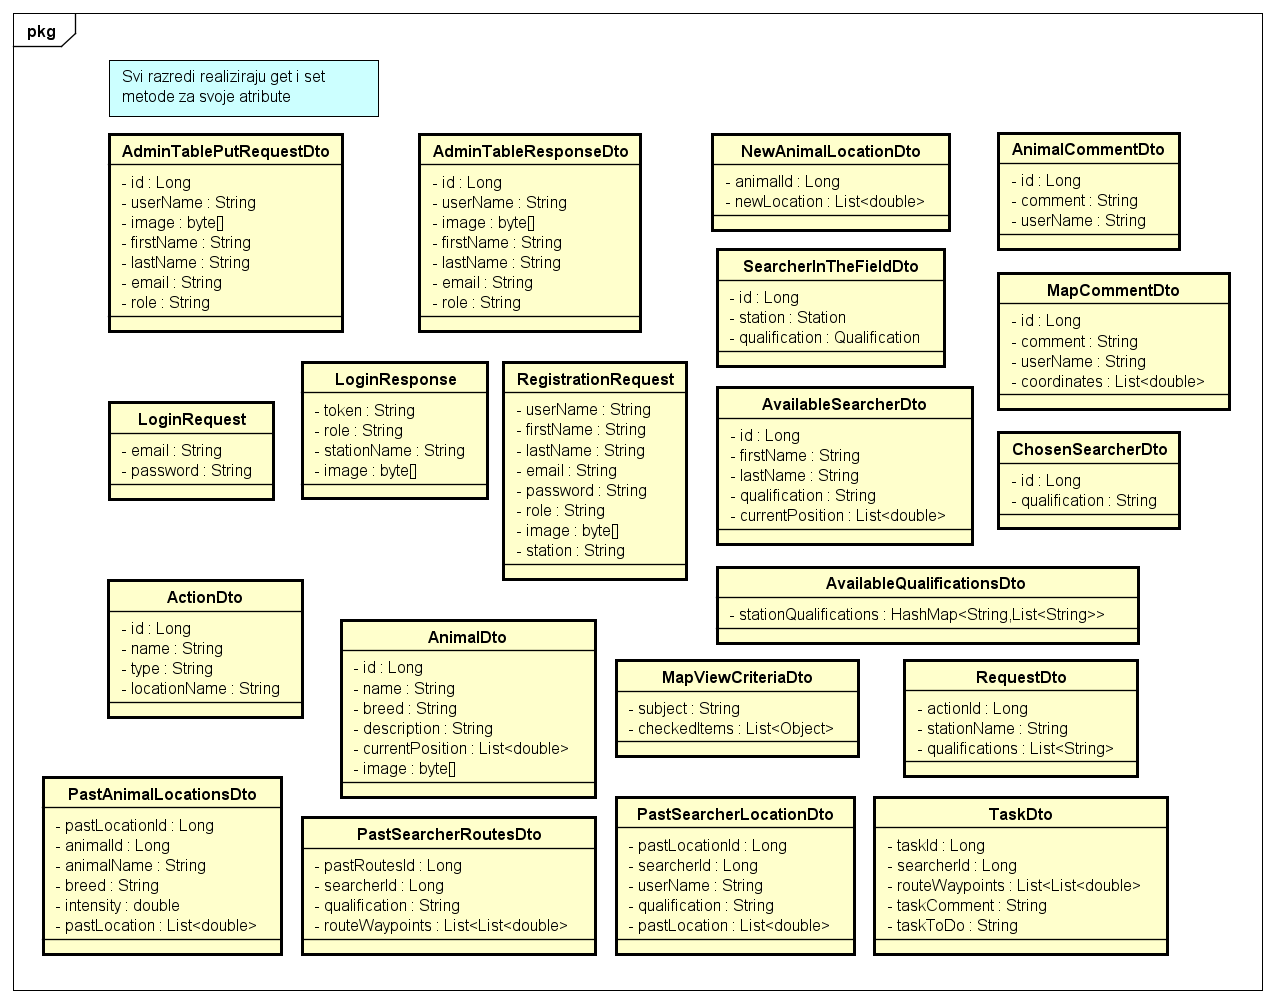
\includegraphics[scale=0.5]{dijagrami/DTO.png} 
				\centering
				\caption{Dijagram razreda - dio DTO}
				\label{fig:promjene}
			\end{figure}
			
			\begin{figure}[H]
				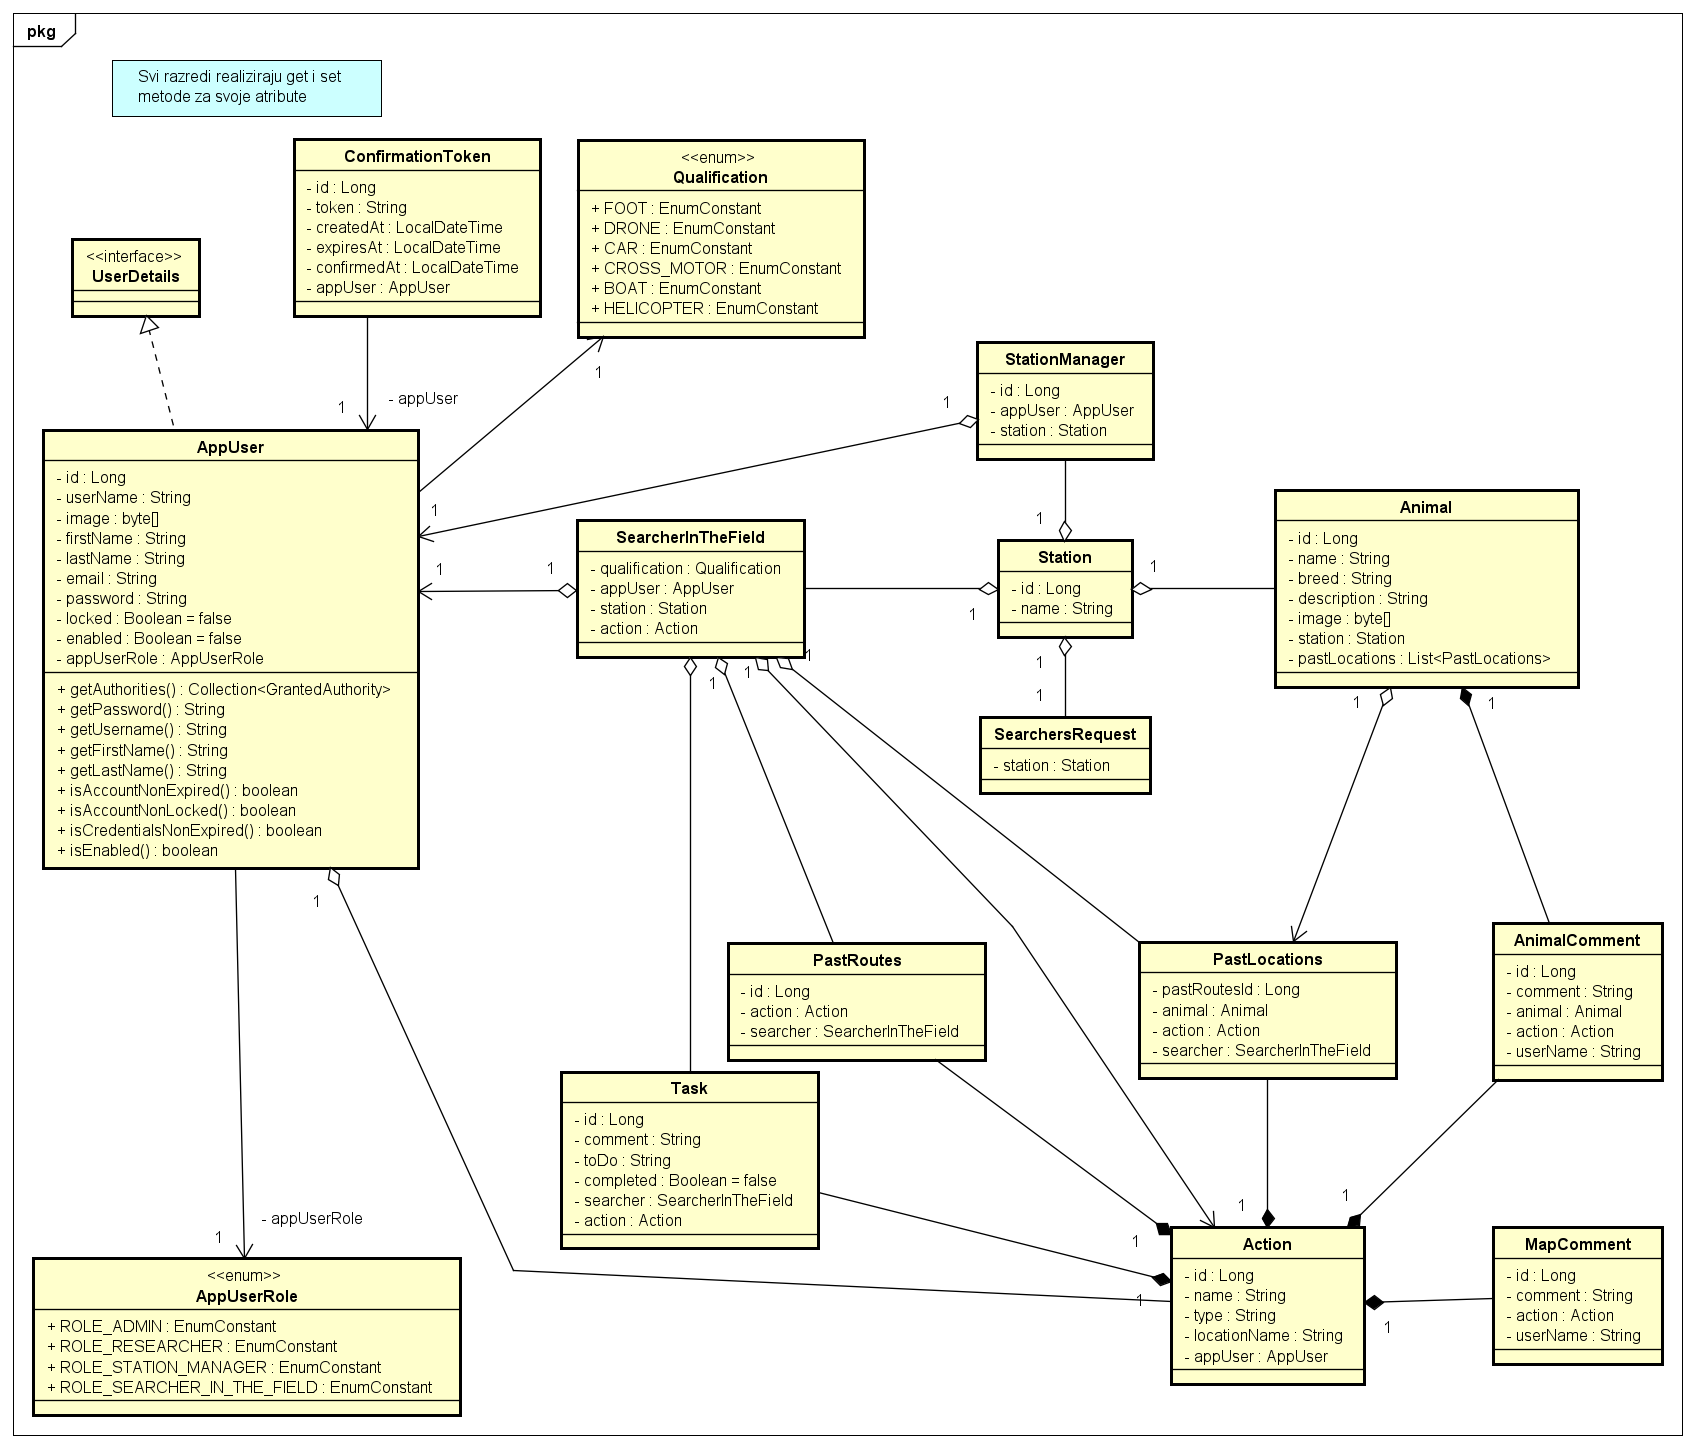
\includegraphics[scale=0.5]{dijagrami/Model.png} 
				\centering
				\caption{Dijagram razreda - dio Models}
				\label{fig:promjene}
			\end{figure}
			
			
			\eject
		
		\section{Dijagram stanja}
			
			
			\textbf{\textit{dio 2. revizije}}\\
			
			\textit{Potrebno je priložiti dijagram stanja i opisati ga. Dovoljan je jedan dijagram stanja koji prikazuje \textbf{značajan dio funkcionalnosti} sustava. Na primjer, stanja korisničkog sučelja i tijek korištenja neke ključne funkcionalnosti jesu značajan dio sustava, a registracija i prijava nisu. }
			
			
			\eject 
		
		\section{Dijagram aktivnosti}
			
			\textbf{\textit{dio 2. revizije}}\\
			
			 \textit{Potrebno je priložiti dijagram aktivnosti s pripadajućim opisom. Dijagram aktivnosti treba prikazivati značajan dio sustava.}
			
			\eject
		\section{Dijagram komponenti}
		
			\textbf{\textit{dio 2. revizije}}\\
		
			 \textit{Potrebno je priložiti dijagram komponenti s pripadajućim opisom. Dijagram komponenti treba prikazivati strukturu cijele aplikacije.}